%%%
%
% $Autor: Wings $
% $Datum: 2021-05-14 $
% $Pfad: Git/MLEdgeComputer/Contents/General/Camov7675 $
% $Dateiname: CAMov2640 
% $Version: 4620 $
%
% !TeX spellcheck = de_GB
%
%%%

\chapter{Sensor ov7675}

\url{https://www.arducam.com/?s=ov7675&id=98994/}

\url{https://www.arducam.com/focal-length-calculator/}

\url{https://docs.arduino.cc/tutorials/giga-r1-wifi/giga-camera/}

\URL{https://blog.arduino.cc/2020/06/24/machine-vision-with-low-cost-camera-modules/}

\URL{https://www.instructables.com/TinyML-Image-Recognition-With-Edge-Impulse-Nano-33/}


\cite{ArduCam:2024}\cite{ArduinoCam:2021b}

\section{Code}

\begin{itemize}
  \item 
  \HREF{https://www.hackster.io/umpheki/ov7670-camera-and-image-sensor-with-nano-33-ble-497c5f}{Arduino sketch} 
   \ArduinoExternalO{../../Code/Arduino/CAM/ov7675/Nano33BLEProgramToReadov7670Data.ino}     
  \item  \HREF{https://www.hackster.io/umpheki/ov7670-camera-and-image-sensor-with-nano-33-ble-497c5f}{save as png}
    \PythonExternalO{../../Code/Arduino/CAM/ov7675/ConvertRawToRGB888AndSaveAspng.py}
  \item  \HREF{https://www.hackster.io/umpheki/ov7670-camera-and-image-sensor-with-nano-33-ble-497c5f}{save as png}
\PythonExternalO{../../Code/Arduino/CAM/ov7675/ReadCameraDataFromNano33BLEViaSerial.py}
\end{itemize}
    
    

\subsection{ OV7670 Camera and Image Sensor with Nano 33 BLE}
 
source: \URL{https://www.hackster.io/umpheki/ov7670-camera-and-image-sensor-with-nano-33-ble-497c5f}

\bigskip

The OV7670 is an image sensor that can be used to capture pictures when controlled by a microprocessor such as the Nano 33 BLE. To quote the datasheet from OmniVision:

“The OV7670/OV7171 CAMERACHIP image sensor is a low voltage CMOS device that provides the full functionality of a single-chip VGA camera and image processor in a small footprint package. The OV7670/OV7171 provides full-frame, sub-sampled or windowed 8-bit images in a wide range of formats, controlled through the Serial Camera Control Bus (SCCB) interface.”

While the OV7670 is a powerful and versatile IC, it produces only Raw pixel data. For most images to be useful, they need to be in jpeg, png, tiff or similar format. This project shows how you can capture a raw image from the camera and then convert this into a png file.

Here are the major components for this project


\begin{itemize}
  \item Arduino Nano 33 BLE
  \item OV7670 camera module
  \item Breadboard
  \item Connectors
  \item Computer with Python ver 3 installed
  
\end{itemize}

\subsubsection{OV7670 CMOS VGA Sensor}

Datasheet for the OV7670 included with this project.

The block diagram from the datasheet:

\begin{center}
  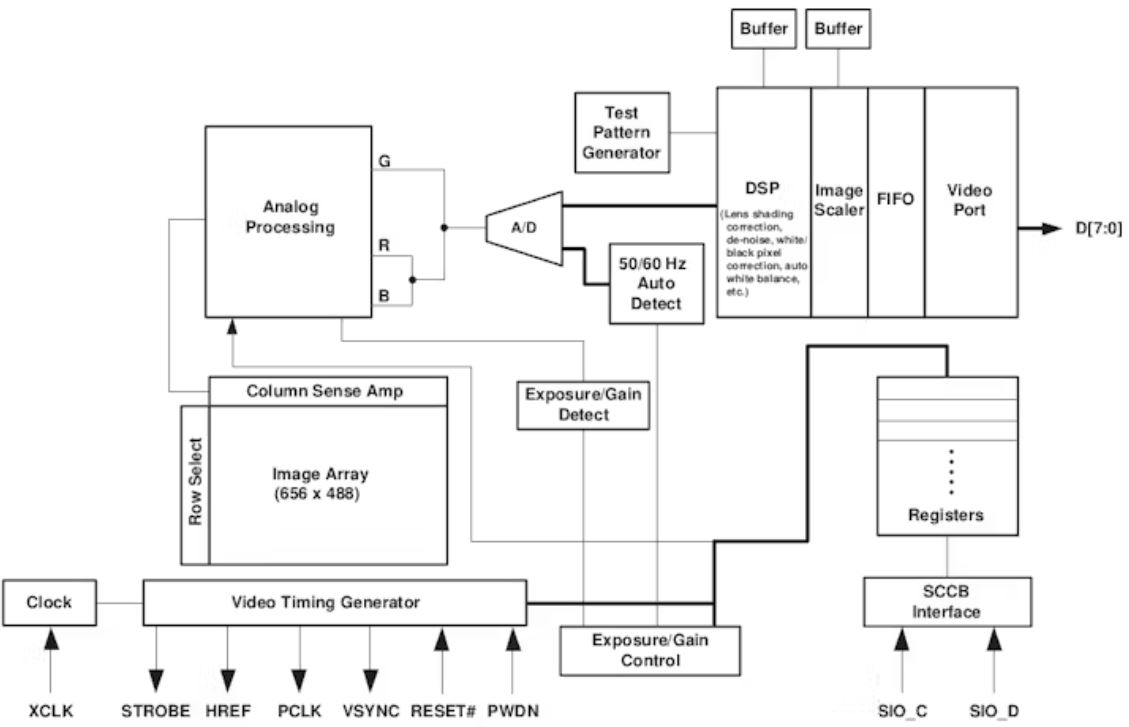
\includegraphics[width=\textwidth]{CAM/ov7675/Blockdiagramm}
  \captionof{figure}{Blockdiagram, der Kamera OV7675}
\end{center}

The image array captures the arriving light and after processing the signal, the signal is converted to a digital signal in a A/D converter. This digital signal can then be read from the data bus (D0 – D7) controlled by SIO\_C and SIO\_D

The OV7670 is capable of capturing video in addition to still images. This project will focus on still images only.

The output formats available from the OV7670 are given on the first page of the datasheet. In this project, the format used is RGB565 (more explanation later)

The image array can take pictures up to 640 x 480 pixels definition. Because of memory limitations on the Nano 33 BLE, pictures up to 320 x 240 are possible (QVGA)

The specific module used in this project includes a simple lens that focuses light on the CMOS array, the focal length of which can be manually adjusted. Loosen the small set screw and twist the lens.


\begin{center}
    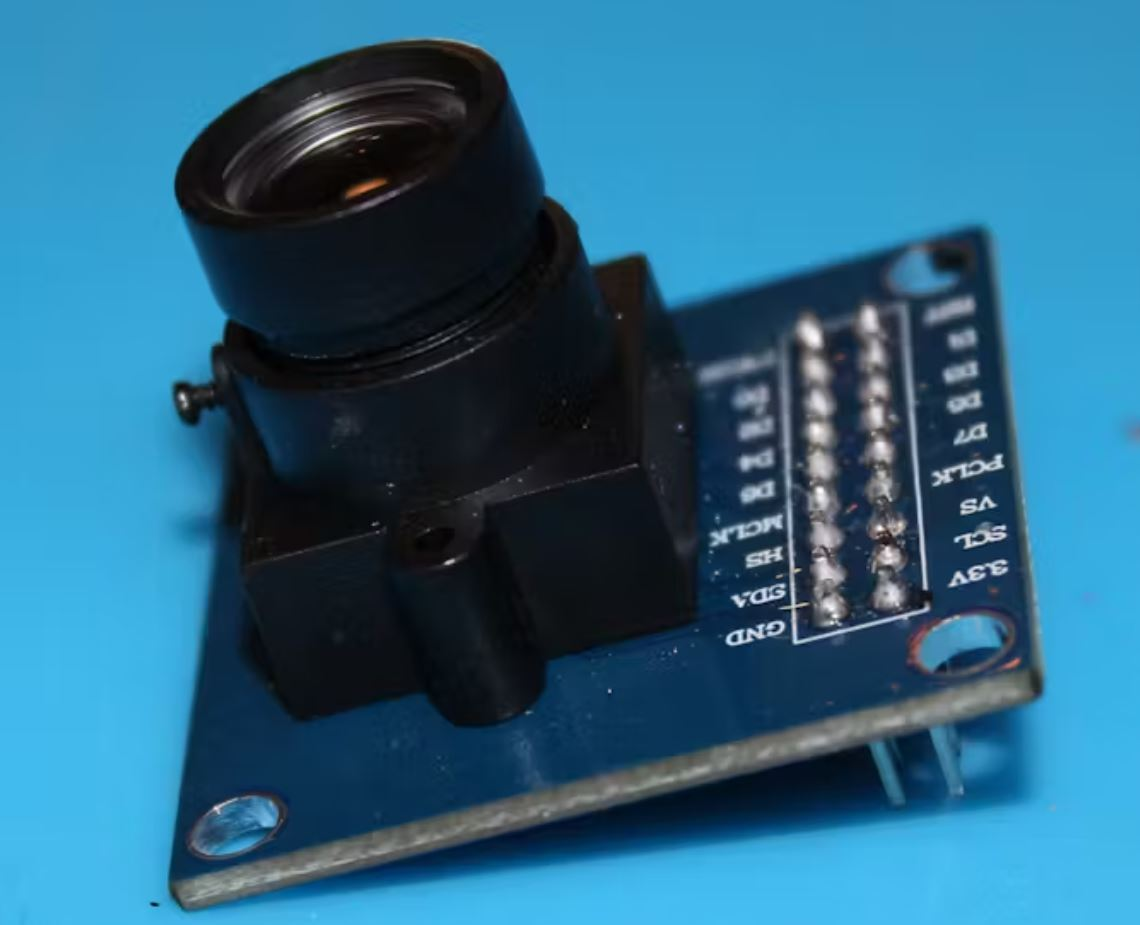
\includegraphics[width=\textwidth]{CAM/ov7675/CameraModule}
    \captionof{figure}{Camera Module OV7675}
\end{center}


\subsection{Connection}

Connection between the Nano and OV7670 as follows

\begin{center}
    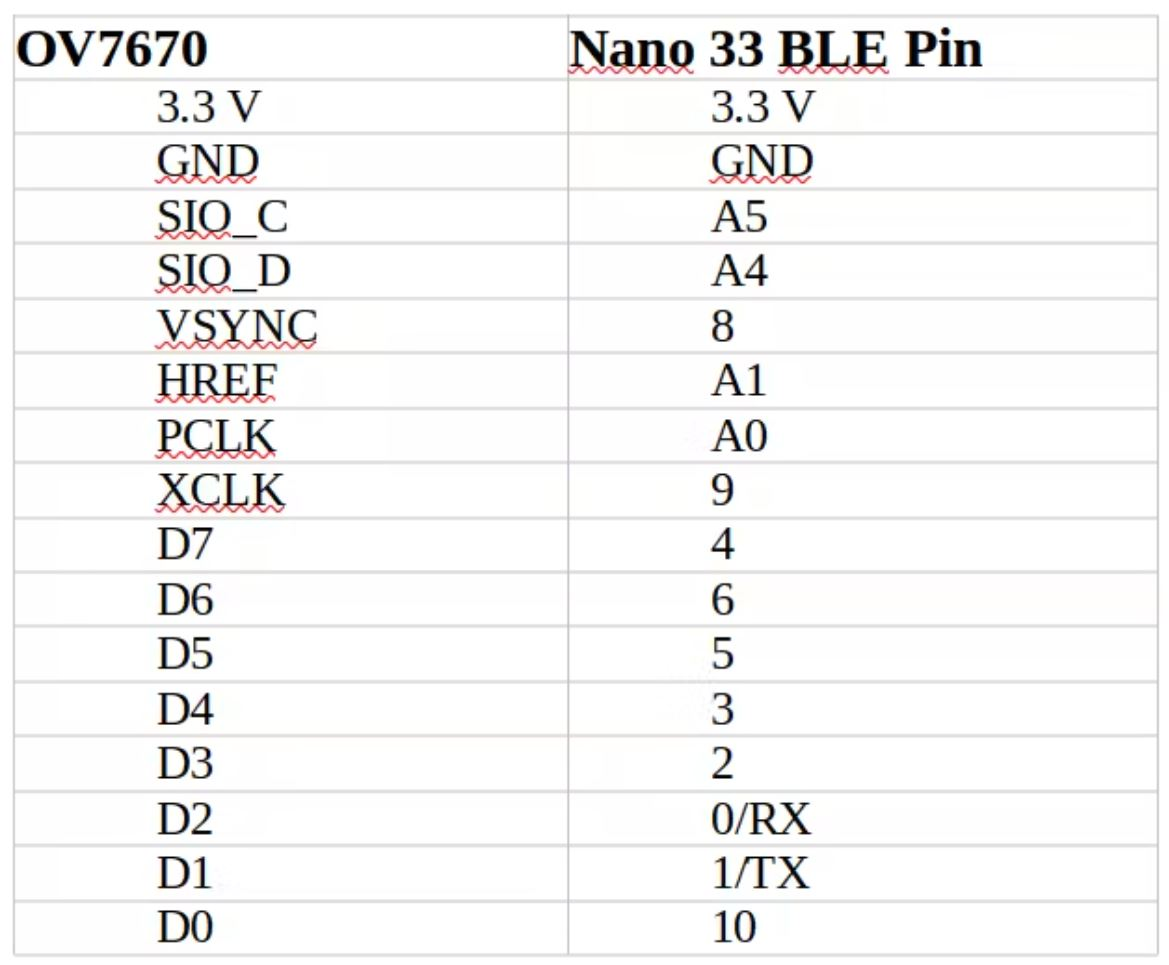
\includegraphics[width=\textwidth]{CAM/ov7675/ConnectionTable}
    \captionof{figure}{Connection Table of the Camera Module OV7675}
\end{center}
    
    
Completing this connection is a little tricky and results in a tangle of wires. Picture included of the final connection

\begin{center}
    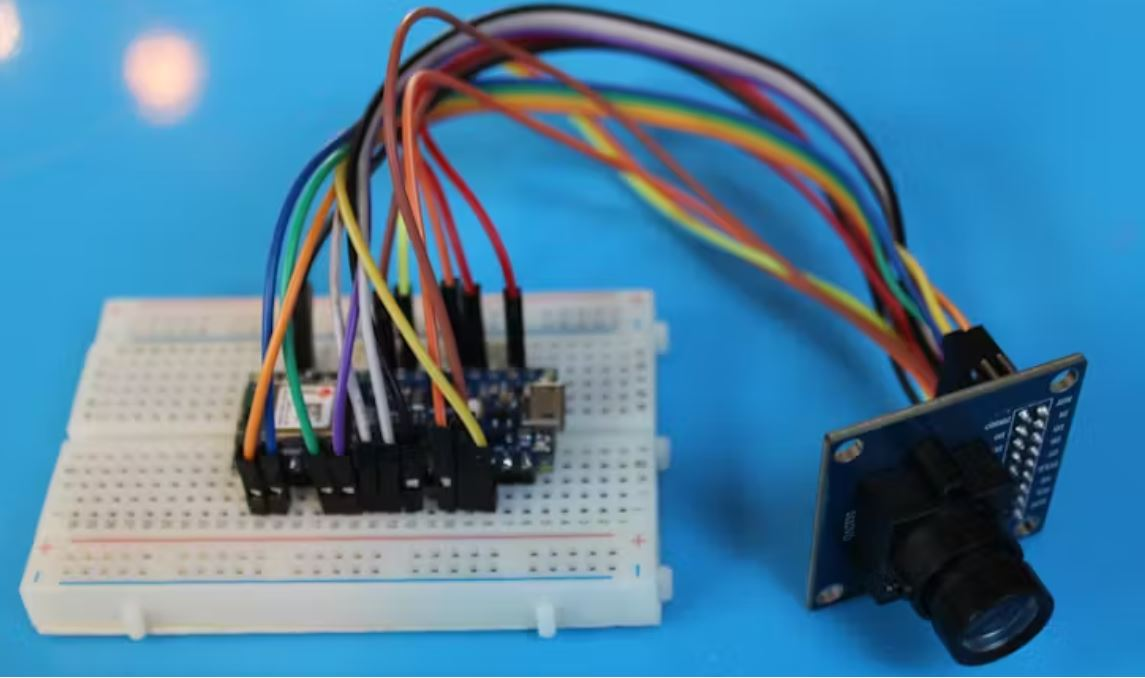
\includegraphics[width=\textwidth]{CAM/ov7675/CameraConnected}
    \captionof{figure}{Camera Module OV7675 connected to the Arduino Nano 33 BLE Sense}
\end{center}
    
    
RGB Formats
In this project, the RGB565 raw format will be used.

If you are interested in a complete explanation of all possible formats, consult the Wikipedia article:

\URL{https://en.wikipedia.org/wiki/List_of_monochrome_and_RGB_color_formats}

Or read this article:

\URL{https://support.touchgfx.com/docs/basic-concepts/color-formats}

RGB565 uses a total of 16 bits as shown    
    
\begin{center}
    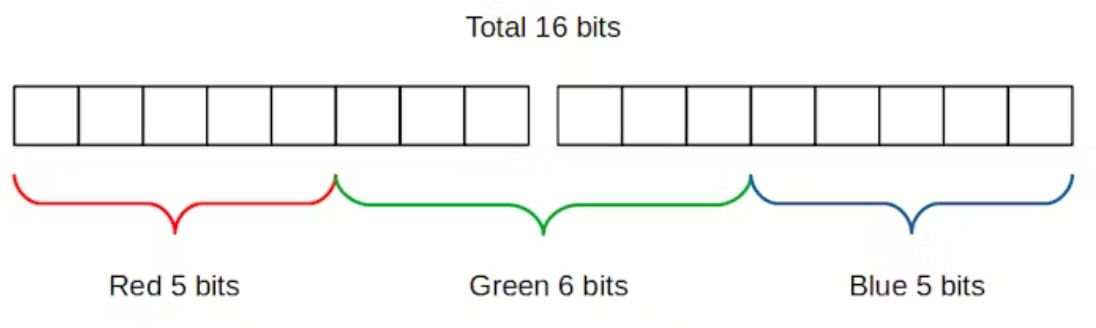
\includegraphics[width=\textwidth]{CAM/ov7675/RGB565}
    \captionof{figure}{RGB565}
\end{center}
    
Green is allocated 6 bits because the human eye is more sensitive to graduations in green than red or blue.

This format was used in the early days of computing when processing and memory was at a premium. Most systems today use RGB888, where each color is allocated 8 bits for a total of 24 bits (so called true color).

This project requires the RGB565 format to be converted to RGB888 format. This is done by a combination of bit shifting and binary masking. The formula to achieve the conversion below:

p = original 16 bit raw 565 pixel information

red component of RGB888 = r = (p >> 11 \& 0b00011111) << 3

green component of RGB888 = g = (p >> 5 \& 0b00111111) << 2

blue component of RGB888 = b = (p >> 0 \& 0b00011111) << 3

To show a specific example, assume a pixel in RGB565 representation which is only red:

p = 11111000 00000000

right shift 11 bits p = 00000000 00011111

bit mask with 0b00011111 p = 00000000 00011111

left shift 3 and drop leading eight bits r = 11111000

Note that the result is not 100\% accurate because low information content cannot be converted to high information content. (However, high information content can always be converted to low information content.)

\subsection{Arduino OV7670 library}
    Before using the OV7670, the Arduino library must be installed.
    
    For Arduino IDE 2.x, search for OV7670 and install the library    
    
\begin{center}
    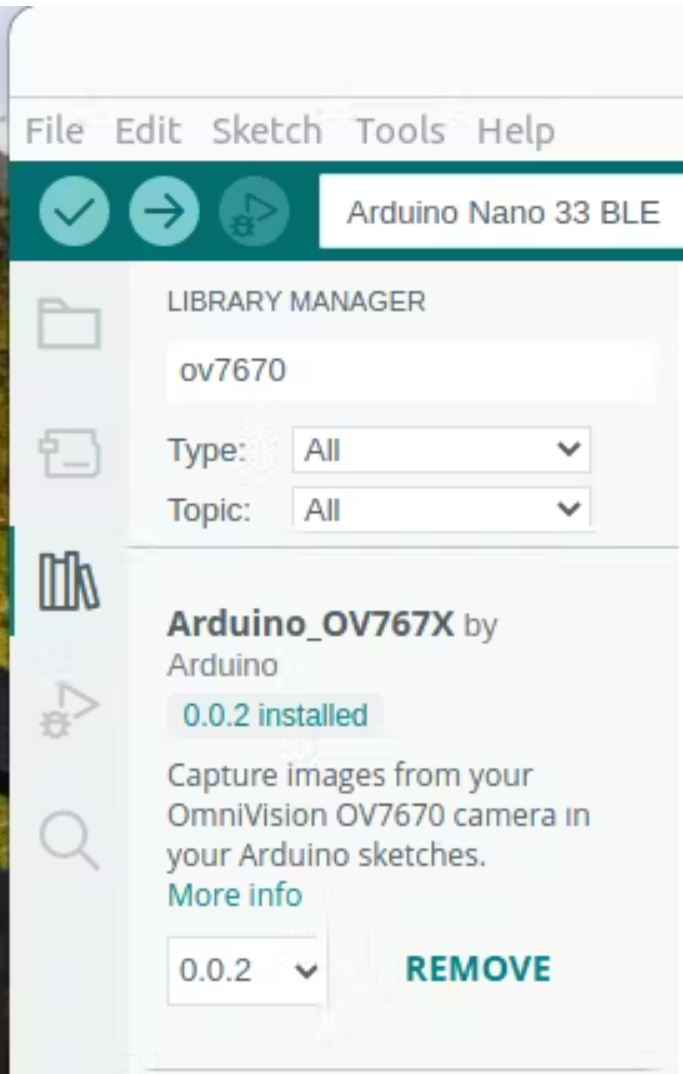
\includegraphics[width=\textwidth]{CAM/ov7675/ArduinoLib}
    \captionof{figure}{Installtion of the Arduino Library}
\end{center}

\subsection{Testing the OV7670}
        
The python program used to read data from the Nano 33 BLE requires that the python library pySerial be installed. This can be installed with the command

\SHELL{pip install pyserial }

(or sudo pip install pyserial, depending on how your computer is configured)

To check if the library is installed use

\SHELL{pip show pyserial}

To test the OV7670, two programs are required. Here are the steps:

\begin{enumerate}
  \item Upload the program “RawCameraCapture.ino” to the Nano 33 BLE
  \item Close the Arduino IDE; the serial monitor in the IDE prevents the python program from communicating with the Nano
  \item Place the camera to point at the subject. Some experimentation with lighting and distance from subject may be required
  \item Navigate to the directory containing the Python program “ReadCamera2.py”
  \item Run the the program with the command
  
        \SHELL{python3 ReadCamera2.py}
  \item Once the process is finished, a message “image transfer complete” will print in the terminal
  \item The program creates a file called “camera” which contains the raw pixel data
  \item Navigate to the website \URL{http://rawpixels.net} in a browser
  \item Upload the file \FILE{camera}
  \item Settings as follows:
    \begin{itemize}
      \item width: 176
      \item height: 144
      \item offset: 0
      \item Predefined Format: RGB565
      \item Pixel Format: RGBA
      \item Ignore Alpha checked
      \item Little Endian not checked
    \end{itemize}
\end{enumerate}

\begin{center}
    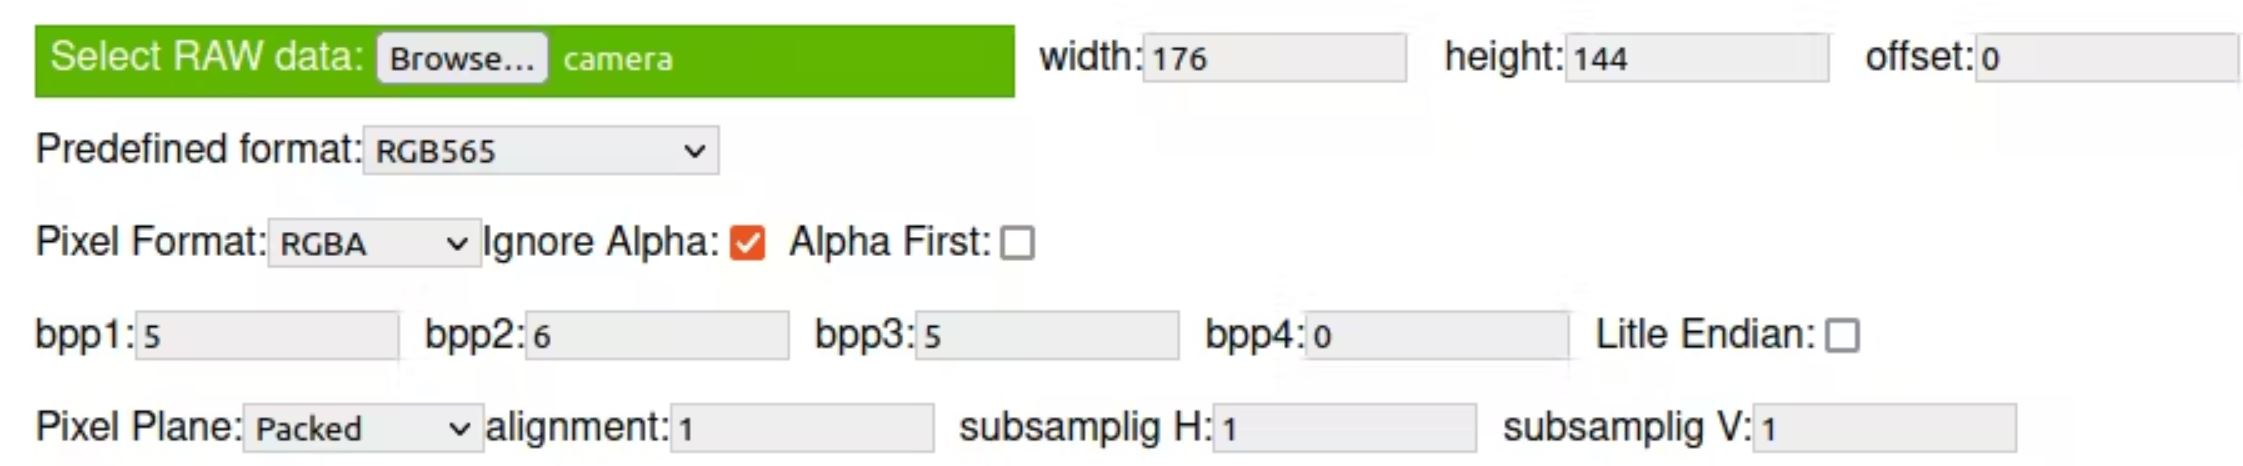
\includegraphics[width=\textwidth]{CAM/ov7675/RawPixelNet}
    \captionof{figure}{Dialogue of RawPixel}
\end{center}
    
The picture should display in the raw pixels interface.

\subsection{Final Step}

Once the test is successful, the final step is to create the PNG image file. Really simple:

\begin{itemize}
  \item Navigate to the directory containing the Python program \FILE{ConvertToPNG.py}
  \item Run the the program with the command
  
       \SHELL{python3 ConvertToPNG.py}
  \item This program creates a temporary RGB888 file called \FILE{imagefile}
  \item A file called \FILE{finalpic.png} will be created    
\end{itemize}
    
\section{Kameramodul OV7675}

\begin{figure}[H]
    \centering
    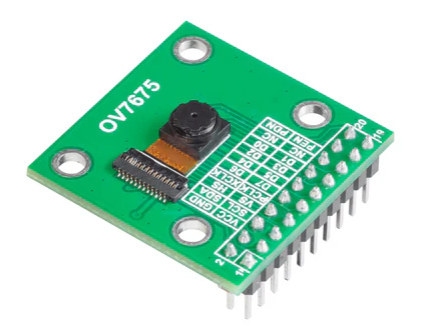
\includegraphics[width=7cm]{CAM/ov7675/modulOV7675}
    \caption{Kameramodul OV7675}
    \label{fig:KameramodulOV7675}
\end{figure}

Um einen Prozess zu überwachen oder ein System zu automatisieren, bietet sich im Rahmen eines Arduino Prozesses das “Arducam 0,3 MP OV7675” Kameramodul \ref{fig:KameramodulOV7675} an, da dieses mit den Arduino Bibliotheken kompatibel ist. Hierbei ist OV7675 die Modellnummer. Der Senor des Moduls verfügt über eine Auflösung von 640 x 480 Pixeln. Die Pixelgröße, die vom Sensor eingefangen werden kann, beträgt 2,5 µm x 2,5 µm. Das Signal-Rausch-Verhältnis, ein Kennwert für die Klarheit des Bildes, beträgt 38 dB. Der Dynamikbereich, welcher angibt, wie Helligkeitsunterschiede erfasst werden können, hat einen Wert von 71 dB. Um Belichtungszeiten zu steuern, verfügt das Modul über elektrische Rollladen. Des Weiteren beinhaltet der Sensor  RGB-Farbfilter (Rot, Grün, Blau).
Daten können über die Formate RAW/YUV/RGB ausgegeben werden. Dies geschieht über einen 20-poligen DVP (Digital Video Port). Verwendet werden darf und kann der Senor in einem Temperaturbereich von –30 °C bis +70 °C. Die Geometrie des Moduls spiegelt sich in der Brettgröße von 30,5 mm x 30,5 mm wider. \cite{Arduino:2024a}


\section{Kamera Modul OV7675}
Um das Kameramodul OV7675 nutzen zu können, muss die Funktion des Bauteils vor Gebrauch getestet werden. Hierzu wird der Sketch TestCameraRawBites320x240x2 \ref{Code:Python:File:TestCameraRawBites320x240x2} ausgeführt.
Folgende Headerdateien werden zum Durchführen des Tests benötigt: $TinyMLShield.h$; $Arduino_OV7675.h$.
Im Test können unterschiedliche Funktionen der Kamera überprüft werden. Dazu gehört der „single“ Befehl. Die Kamera nimmt ein einzelnes Bild auf, wenn im Nachhinein der Befehl capture geschrieben wird. Dadurch gibt das Programm Hexadezimalwerte für jeden Pixel des Bildes aus. In diesem Fall muss der ausgegebene Text in Google Colab eingefügt werden, sodass aus der Sequenz im serieller Monitor ein Bild konvertiert werden kann.
Die Funktion „live“ streamt die Bytes der aufgenommenen Bilder über die serielle Schnittstelle.
Der Befehl „capture“ löst im single-Modus eine einzelne Bildschirmaufnahme aus.

Um live Übertragungen des Kamera-Moduls streamen zu können, was für unser Projekt essentiell  ist, wird ein weiteres Programm „Processing“ benötigt. Dieses wird auf dem Endgerät installiert.

\section{header}
Der Header dieses Codes \ref{Code:Python:File:TestENCheader} richtet die Ethernet Verbindung mit den Bibliotheken <SPI.h> und <EthernetENC.h> ein. Außerdem werden die Makros ON und OFF deklariert. Die Ip Adresse wird zugewiesen und der Server, über den HTTP-Anfragen empfangen und Antworten gesendet werden, wird auf Port 80 gesetzt.

\begin{code}
    \lstinputlisting[language=c++]{../../Code/Arduino/CAM/ov7675/TestENCheader.ino}    
    \caption[Sketch  \FILE{TestENCheader.ino}]{Der Sketch  \FILE{TestENCheader.ino} in Arduino für das Microcontroller Board}
    \label{Code:Python:File:TestENCheader}    
\end{code} 

\section{\PYTHON{void setup()}}

Im Void Setup \ref{Code:Python:File:TestENCVoidSetup} wird eine Sequenz für die LED festgelegt, um den Betriebsstatus sichtbar zu machen. Die Ethernet-Verbindung wird aufgebaut und mögliche Fehler werden im seriellen Monitor ausgegeben.

\begin{code}[H]
    \lstinputlisting[language=c++]{../../Code/Arduino/CAM/ov7675/TestENCVoidSetup.ino}    
    \caption[Sketch  \FILE{TestENCVoidSetup.ino}]{Der Sketch  \FILE{TestENCVoidSetup.ino} in Arduino für das Microcontroller Board}
    \label{Code:Python:File:TestENCVoidSetup}    
\end{code} 

\section{\PYTHON{void loop()}}

In der Funktion \PYTHON{loop} \ref{Code:Python:File:TestENCVoidLoop} befindet sich der Hauptteil des einfachen Webservers, der über HTTP kommuniziert und zur Funktionsprüfung eine LED ansteuert.

\begin{code}
    \lstinputlisting[language=c++]{../../Code/Arduino/CAM/ov7675/TestENCVoidLoop.ino}    
    \caption[Sketch  \FILE{TestENCVoidLoop.ino}]{Der Sketch  \FILE{TestENCVoidLoop.ino} in Arduino für das Microcontroller Board}
    \label{Code:Python:File:TestENCVoidLoop}    
\end{code} 




\section{Test der Bildaufnahme} 
Mit diesem Code \ref{Code:Python:File:TestCameraRawBites320x240x2} und der dazugehörigen Bibliothek <Arduino OV767X.h> wird die Kamera angesteuert. Bei jedem aufgenommenen Bild überträgt die Kamera 1.228.800 Bits kontinuierlich über die serielle Schnittstelle an den Computer. Außerdem wurde die grüne LED mit implementiert, um den Betriebsstatus anzuzeigen und eine mögliche Fehlersuche zu vereinfachen.
\begin{code}
    \lstinputlisting[language=c++]{../../Code/Arduino/CAM/ov7675/TestCameraRawBites320x240x2.ino}
    \caption[Sketch \FILE{TestCameraRawBites320x240x2.ino}]{Der Sketch \FILE{TestCameraRawBites320x240x2.ino} in Arduino für das Microcontroller Board}
    \label{Code:Python:File:TestCameraRawBites320x240x2}   
\end{code}

\section{Bildverarbeitung} 

In der Processing Anwendung werden die seriell übertragenen Daten vom Processing Skript \ref{Code:Python:File:CameraVisualizerHochkant320x240x2} verarbeitet und um 90 Grad nach links gedreht. Somit wird das live Bild in einem kleinen Fenster gestreamt \ref{fig:Bildschirmaufnahme} .

\begin{figure}
    \centering
    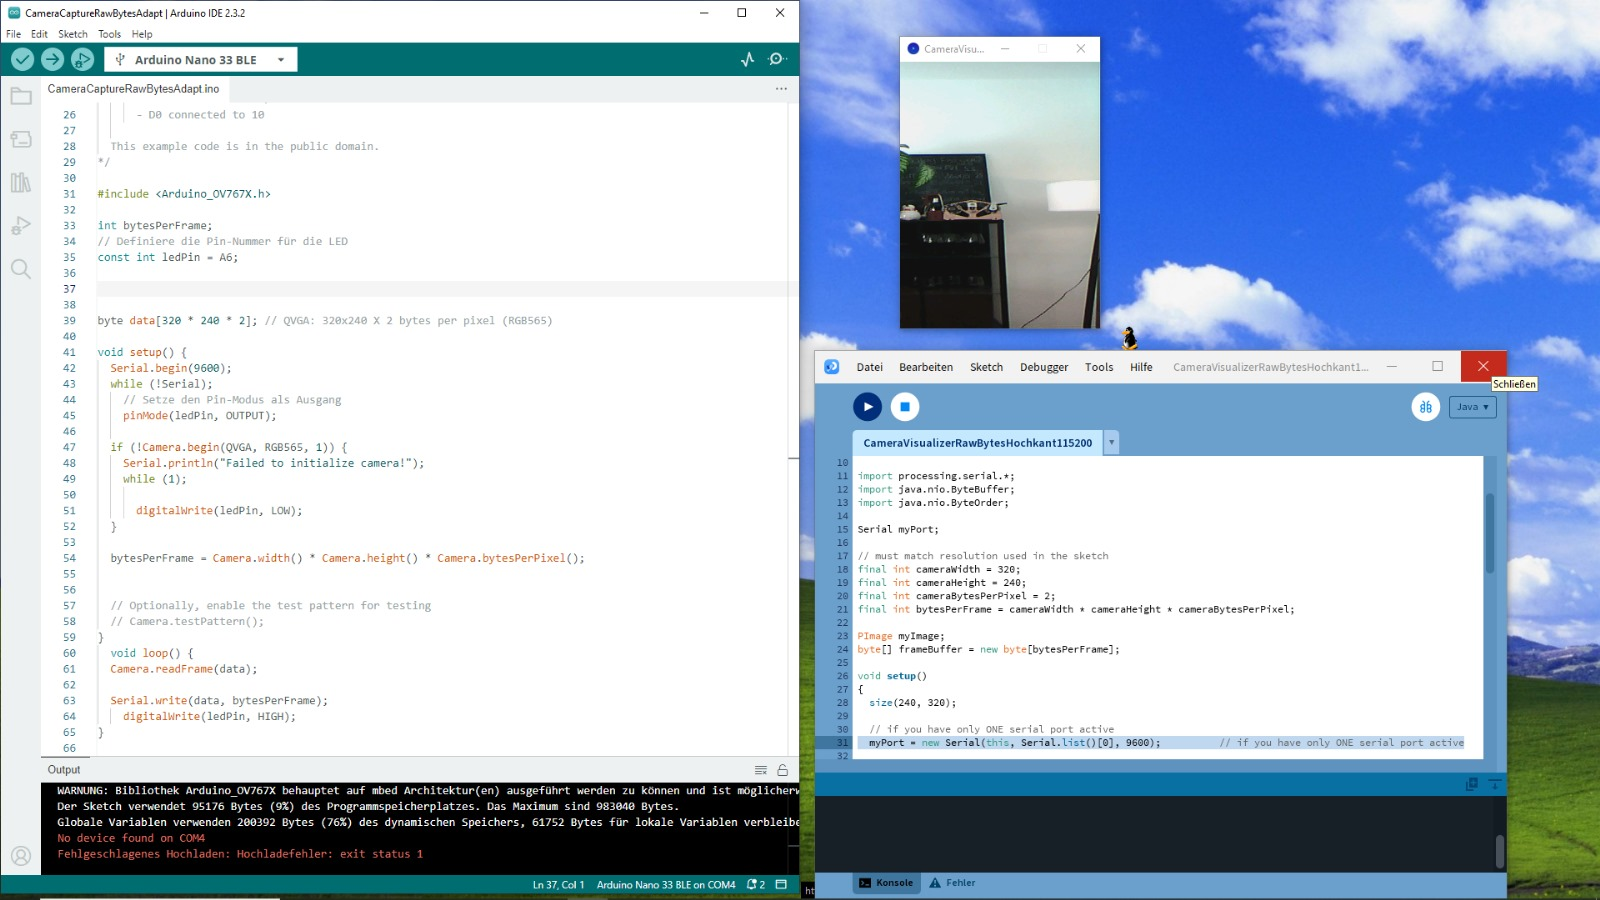
\includegraphics[width=10cm]{CAM/ov7675/Screenshot}
    \caption{Bildschirmaufnahme}
    \label{fig:Bildschirmaufnahme}
\end{figure}

\begin{code}
    \lstinputlisting[language=python]{../../Code/Arduino/CAM/ov7675/CameraVisualizerHochkant320x240x2.ino}
    \caption[Sketch \FILE{CameraVisualizerHochkant320x240x2.ino}]{Der Sketch \FILE{CameraVisualizerHochkant320x240x2.ino} in Arduino für das Microcontroller Board}
    \label{Code:Python:File:CameraVisualizerHochkant320x240x2}   
\end{code}


%%%%%%%%%%%%%%%%%%%%%%%%%%%%%%%%%%%%%%%%%%%%%%%%%%%%%%%%%%%%%%%%%%%%%%%%

\section{Produktbeschreibung}

Arducam-M-2MP ist eine optimierte Version von Arducam Shield Rev.C und ist eine hochauflösende 2MP-SPI-Kamera, die die Komplexität der Kamerasteuerung verringert. Sie verfügt über einen 2-MP-CMOS-Bildsensor OV2640 und hat eine Miniaturgröße sowie eine einfach zu bedienende Hardware-Schnittstelle und die Open-Source-Code-Bibliothek. Die Arducam Mini-Kamera kann auf allen Plattformen wie Arduino, Raspberry Pi, Maple, Chipkit, Beaglebone Black verwendet werden, solange sie über eine SPI- und I2C-Schnittstelle verfügen und mit Standard-Arduino Boards verbunden werden können. Die Arducam Mini-Kamera bietet nicht nur die Möglichkeit, eine Kamera-Schnittstelle hinzuzufügen, die in einigen Mikrocontrollern nicht vorhanden ist, sondern bietet auch die Möglichkeit, mehrere Kameras zu einem einzigen Mikrocontroller hinzuzufügen.
\Mynote{Plagiat! cite!}
\bigskip

Anwendung:

\begin{itemize}
  \item IoT-Kameras.
  \item Roboterkameras.
  \item Wildlife-Kameras.
\end{itemize}

Andere batteriebetriebene Produkte.

Kann auf Plattformen wie MCU, Raspberry Pi, ARM, DSP, FPGA verwendet werden.

\bigskip

Eigenschaften:

\begin{itemize}
  \item 2-Megapixel-Bildsensor OV2640.
  \item M12-Mount- oder CS-Mount-Objektivhalter mit wechselbaren Objektivoptionen.
  \item IR-empfindlich mit entsprechender Objektivkombination.
  \item I2C-Schnittstelle für die Sensorkonfiguration.
  \item SPI-Schnittstelle für Kamera-Befehle und Datenstrom.
  \item Alle E/A-Anschlüsse sind für 5 V/3,3 V geeignet.
  \item Unterstützt JPEG-Komprimierungsmodus, Einzel- und Mehrfachaufnahmemodus, einmaliges Erfassen mehrerer Lesevorgänge, Burst-Lese-Operation, Niedrige-Energie-Modus usw..
  \item Kann mit Standard-Arduino-Boards verbunden werden.
  \item Open-Source-Code-Bibliothek für Arduino, STM32, Chipkit, Raspberry Pi, BeagleBone Black.
  \item Schlanke Form.
\end{itemize}

\bigskip

Lieferumfang:

1 x Arducam Mini-Modul Kameraschutz mit OV2640 2 MP, Objektiv, für Arduino UNO Mega2560 Board.

Hinweis: Arduino UNO ist nicht enthalten.

\bigskip


\url{https://www.amazon.com/dp/B07D58GDDV/ref=sr_1_17_sspa?__mk_de_DE=ÅMÅŽÕÑ&dchild=1&keywords=arducam&qid=1622358684&sr=8-17-spons&psc=1&spLa=ZW5jcnlwdGVkUXVhbGlmaWVyPUEyWUdNSVhJSFNUQUtLJmVuY3J5cHRlZElkPUEwNjI4NTQxM0RNQ0I2NDJDNzdUTCZlbmNyeXB0ZWRBZElkPUEwMjEyMjUwNTFSVjM2SzZFM1VCJndpZGdldE5hbWU9c3BfYXRmX25leHQmYWN0aW9uPWNsaWNrUmVkaXJlY3QmZG9Ob3RMb2dDbGljaz10cnVl0}

    
Raspberry Pi Kamerakabel, iUniker 15-poliges Flachbandkabel, Pi Kamera Flex Kabel, Flex CSI Kabel 50 cm/1 m/2 m für Raspberry Pi 3B+, 3B, 2B (nicht für Pi Zero)
    
\begin{figure}
    \begin{center}
        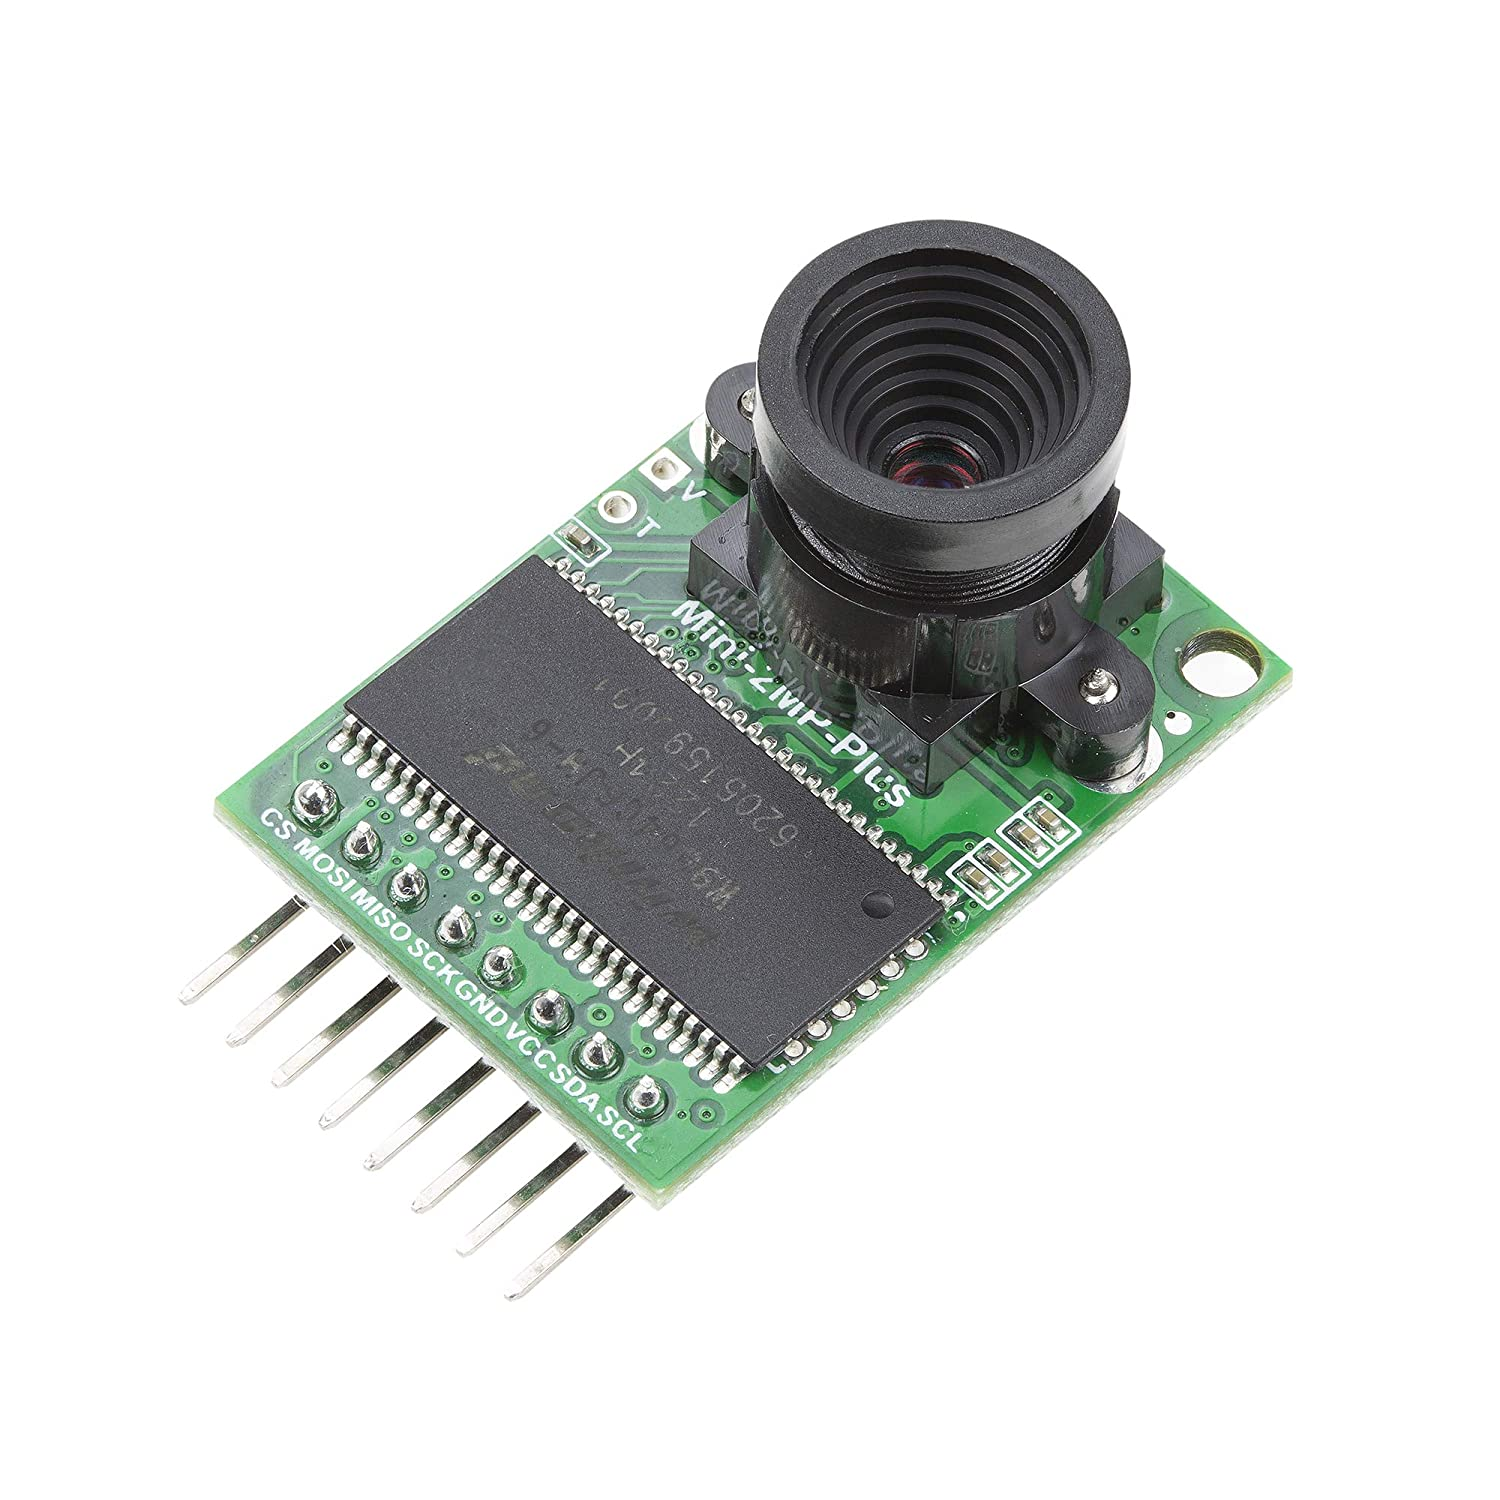
\includegraphics[scale=0.13]{CAM/ov2640/ov2640}
        \quad 
        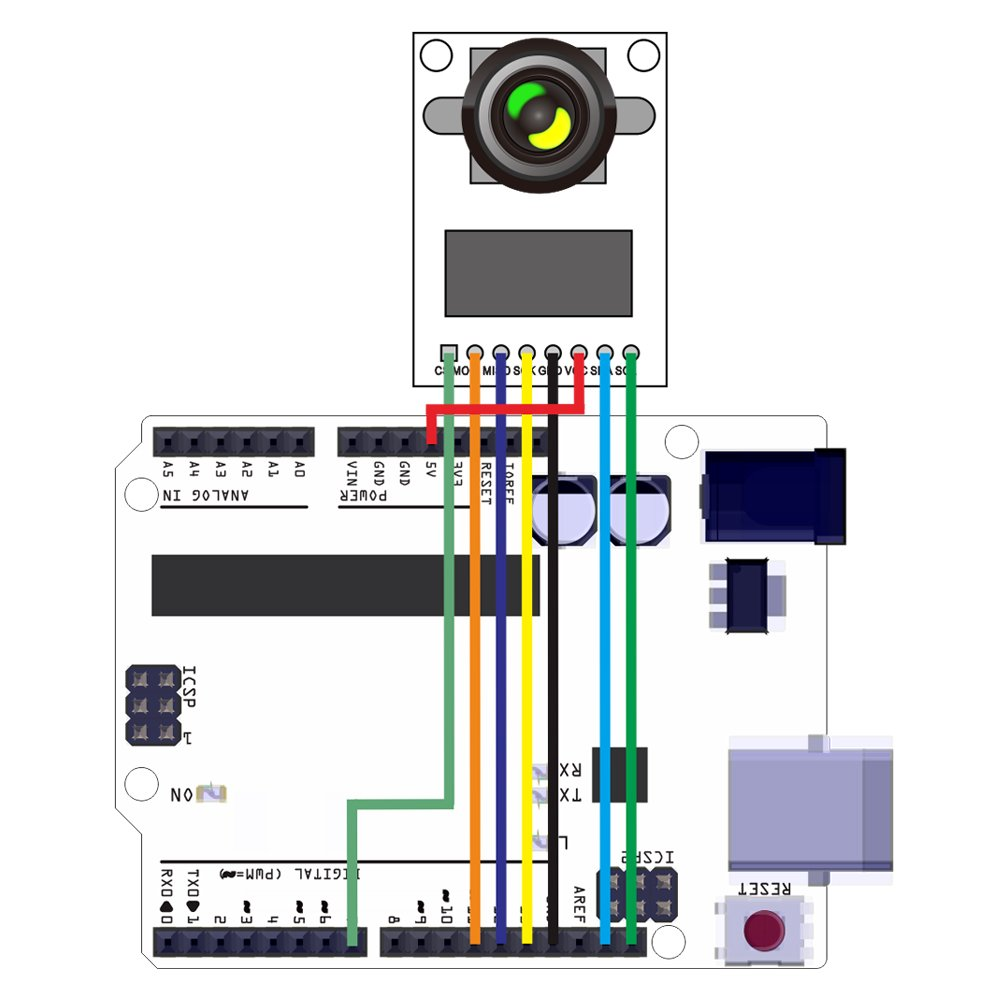
\includegraphics[scale=0.15]{CAM/ov2640/ov2640B4}
        
        \caption{Kamera IMX477 der Firma Arducam; \cite{Arducam:2021}}
    \end{center}    
\end{figure}



\section{ArduCAM Library Introduction}

\url{https://github.com/ArduCAM/Arduino}


Dies ist eine Open-Source-Bibliothek für die Aufnahme von hochauflösenden Standbildern und kurzen Videoclips auf Arduino-basierten Plattformen unter Verwendung der Kameramodule von ArduCAM.
Die Kamera-Breakout-Boards sollten vor dem Anschluss an die Arduino-Boards mit dem ArduCAM-Shield funktionieren.
ArduCAM-Kameramodule der Mini-Serie wie Mini-2MP, Mini-5MP(Plus) können direkt an Arduino-Boards angeschlossen werden.
Zusätzlich zu Arduino kann die Bibliothek auf beliebige Hardware-Plattformen portiert werden, solange sie über eine I2C- und SPI-Schnittstelle verfügen, die auf dieser ArduCAM-Bibliothek basiert.

\bigskip

Now Supported Cameras

\begin{itemize}
  \item OV7660 0.3MP
  \item OV7670 0.3MP
  \item OV7675 0.3MP
  \item OV7725 0.3MP
  \item MT9V111 0.3MP
  \item MT9M112 1.3MP
  \item MT9M001 1.3MP
  \item MT9D111 2MP
  \item OV2640 2MP JPEG
  \item MT9T112 3MP
  \item OV3640 3MP
  \item OV5642 5MP JPEG
  \item OV5640 5MP JPEG
\end{itemize}

Supported MCU Platform

Theoretically support all Arduino families

\begin{itemize}
  \item Arduino UNO R3 (Tested)
  \item Arduino MEGA2560 R3 (Tested)
  \item Arduino Leonardo R3 (Tested)
  \item Arduino Nano (Tested)
  \item Arduino DUE (Tested)
  \item Arduino Genuion 101 (Tested)
  \item Raspberry Pi (Tested)
  \item ESP8266-12 (Tested) (\url{http://www.arducam.com/downloads/ESP8266_UNO/package_ArduCAM_index.json})
  \item Feather M0 (Tested with OV5642)
\end{itemize}


Note: ArduCAM library for ESP8266 is maintained in another repository ESP8266 using a json board manager script.


\section{Libraries Structure}

Die Basisbibliotheken bestehen aus zwei Unterbibliotheken: \FILE{ArduCAM} und \FILE{UTFT4ArduCAM\_SPI}. Diese beiden Bibliotheken sollten direkt unter die Bibliotheken des Arduino-Verzeichnisses kopiert werden, damit sie von der Arduino-IDE erkannt werden.

Die ArduCAM-Bibliothek ist die Kernbibliothek für ArduCAM-Shields. Sie enthält unterstützte Bildsensortreiber und Benutzerland-API-Funktionen, die Befehle zum Erfassen oder Lesen von Bilddaten erteilen. Es gibt auch ein Beispielverzeichnis innerhalb der ArduCAM-Bibliothek, das die meisten Funktionen der ArduCAM-Shields illustriert. Die vorhandenen Beispiele sind Plug-and-Play, ohne dass eine einzige Zeile Code geschrieben werden muss.

Die Bibliothek \FILE{UTFT4ArduCAM\_SPI} ist eine modifizierte Version von UTFT, die von Henning Karlsen geschrieben wurde. Wir haben sie portiert, um das ArduCAM-Shield mit LCD-Bildschirm zu unterstützen. Daher wird die Bibliothek \FILE{UTFT4ArduCAM\_SPI} nur benötigt, wenn das ArduCAM-LF-Modell verwendet wird.




\section{How to use}

Die Bibliotheken sollten vor dem Ausführen von Beispielen konfiguriert werden, andernfalls erhalten Sie eine Fehlermeldung beim Kompilieren.

\subsection{1. Edit \FILE{memorysaver.h} file}

Öffnen Sie die Datei \FILE{memorysaver.h} im ArduCAM-Ordner und aktivieren Sie die Hardwareplattform und das Kameramodul, das zu Ihrer Hardware passt, indem Sie die Makrodefinition in der Datei auskommentieren oder auskommentieren. Wenn Sie zum Beispiel eine ArduCAM-Mini-2MP haben, sollten Sie die Zeile \PYTHON{\#define OV2640\_MINI\_2MP} auskommentieren und alle anderen Zeilen auskommentieren. Und wenn Sie ein ArduCAM-Shield-V2 und ein OV5642-Kameramodul haben, sollten Sie die Zeile \PYTHON{\#define ARDUCAM\_SHIELD\_V2} und die Zeile \PYTHON{\#define OV5642\_CAM} auskommentieren und dann alle anderen Zeilen.

\subsection{2. Choose correct CS pin for your camera}

Öffnen Sie eines der Beispiele und verdrahten Sie die SPI- und I2C-Schnittstelle, insbesondere die CS-Pins, entsprechend den Beispielen mit dem ArduCAM-Shield. Hardware und Software sollten konsistent sein, um die Beispiele korrekt auszuführen.

\subsection{3. Upload the examples}


Im Beispielordner befinden sich sieben Unterverzeichnisse für verschiedene ArduCAM-Modelle und die Host-Anwendung. Der Ordner Mini ist für die Module ArduCAM-Mini-2MP und ArduCAM-Mini-5MP.

\begin{enumerate}
  \item Der Ordner \FILE{Mini\_5MP\_Plus} ist für ArduCAM-Mini-5MP-Plus (OV5640/OV5642) Module.
  \item Der Ordner \FILE{RevC} ist für ArduCAM-Shield-RevC oder ArduCAM-Shield-RevC+ Shields.
  \item Der Ordner \FILE{Shield\_V2} ist für das ArduCAM-Shield-V2 Schild.
  \item Der Ordner \FILE{host\_app} ist die Host-Erfassungs- und Anzeigeanwendung für alle ArduCAM-Module.
  \item Der Ordner \FILE{RaspberryPi} ist eine Beispielanwendung für die Raspberry Pi-Plattform, siehe weitere Anleitung.
  \item Der Ordner \FILE{ESP8266} ist für ArduCAM-ESP8266-UNO-Board-Beispiele für Bibliothekskompatibilität. Bitte versuchen Sie stattdessen, ESP8266 mit dem Skript josn board manager zu repositoryen.
\end{enumerate}


Selecting correct COM port and Arduino boards then upload the sketches.

\bigskip

     
Arducam MINI Kamera Demo Tutorial für Arduino

Arducam Kamera-Schild V2 Demo Tutorial für Arduino

\subsection{4. How To Connect Bluetooth Module}
Mit dieser Demo

\url{https://github.com/ArduCAM/Arduino/blob/master/ArduCAM/examples/mini/ArduCAM_Mini_Video_Streaming_Bluetooth}

So laden Sie den Host V2:

% \Ausblenden
{

\begin{itemize}
  \item For ArduCAM\_Host\_V2.0\_Mac.app, please refer to this link:
  
         \url{www.arducam.com/downloads/app/ArduCAM_Host_V2.0_Mac.app.zip}
  \item For ArduCAM\_Mini\_V2.0\_Linux\_x86\_64bit, Please refer to this link:
       
       \url{www.arducam.com/downloads/app/ArduCAM_Mini_V2.0_Linux_x86_64bit.zip}
\end{itemize}

}
